	Esse capítulo tem como objetivo, descrever todo o processo de desenvolvimento realizado para detectar possíveis fraudes na CEAP. Inicialmente descrevo em detalhes como foi desenvolvido um ETL para extrair os dados da CEAP, fornecidos pela câmara dos deputados, e carregá-los no OrientDB, além de explicar a modelagem feita para o armazenamento dos dados. Em seguida, explico o funcionamento das consultas realizadas para a detecção de fraudes. Finalmente, apresento a arquitetura do sistema web, e como o sistema se comunica com o OrientDB e apresenta informações relevantes sobre os dados.

\section{ETL e modelo do banco de dados}

\subsection{Dados Abertos}

Foram utilizadas duas bases de dados abertos para o desenvolvimento deste trabalho. A primeira é referente aos dados da cota para exercício da atividade parlamentar, e pode ser obtida no seguinte site da Câmara dos Deputados\footnote{http://www2.camara.leg.br/transparencia/cota-para-exercicio-da-atividade-parlamentar/dados-abertos-cota-parlamentar}. A segunda base diz respeito as doações que cada deputado recebeu de empresas ou pessoas físicas, para a campanha eleitoral de 2014, e pode ser obtida no seguinte site do Tribunal Superior Eleitoral \footnote{http://www.tse.jus.br/eleitor-e-eleicoes/estatisticas/repositorio-de-dados-eleitorais-1/repositorio-de-dados-eleitorais}.

A iniciativa de disponibilizar dados e informações por meio de portais tem como um dos objetivos melhorar a confiança da população nos serviços prestados pelo governo. A transparência governamental é , portanto, uma ótima iniciativa e extremamente benéfica para a população. Porém ainda existem diversos pontos a serem melhorados para que estudos sejam feitos de forma mais rápida e precisa. Um dos maiores desafios desse projeto foi trabalhar com as bases de dados abertas mencionadas nessa seção.

Trabalhar com esses dados abertos se tornou um desafio, porque, cada instituição fornece os dados da própria maneira, essa falta de padronização dificultou bastante a fase de carregamento dos dados. Isso se deve ao fato de que a base de dados do TSE fornece o cpf de cada candidato, já a base da CEAP não fornece um identificador único para o deputado. Portanto, no momento de realizar o cruzamento não existia um identificador único em ambas as bases para fazer o relacionamento entre as bases de dados. Para resolver esse problema, se fez necessário realizar o cruzamento entre as bases por meio do nome de cada candidato, o que também foi um desafio, já que cada base utiliza um nome diferente para cada candidato. Os detalhes do processo de extração, transformação e carregamento serão fornecidos na Seção \ref{etl-subsection}, o ponto principal a ser levantado é que trabalhar com dados abertos no Brasil, para realizar estudos e pesquisas, pode se tornar um desafio devido a falta de padronização entre as bases de dados. 

\subsection{Modelo de dados}

A modelagem dos dados seguiu o modelo GRAPHED \cite{graphed}. O trabalho em questão, busca propor formas de modelagem dos dados para bancos de dados orientado a grafos, uma área já desenvolvida no universo dos SGBD relacionais, mas ainda em evolução na categoria de SGBD orientado a grafos.

A modelagem tem como objetivo dar uma visão geral de como os dados estão organizados no banco de dados, suas propriedades e relacionamentos. Dessa forma, o modelo de dados desenvolvido busca evidenciar as propriedades dos parlamentares, tais como: nome, partido e unidade federativa. Além disso apresenta características que identificam uma empresa como nome e CNPJ, e características atreladas a transação que o deputado faz com uma empresa como o valor e descrição da transação. A Figura \ref{fig:modeloDeDados} apresenta a modelagem  desenvolvida.

\begin{figure}[H]
\centering
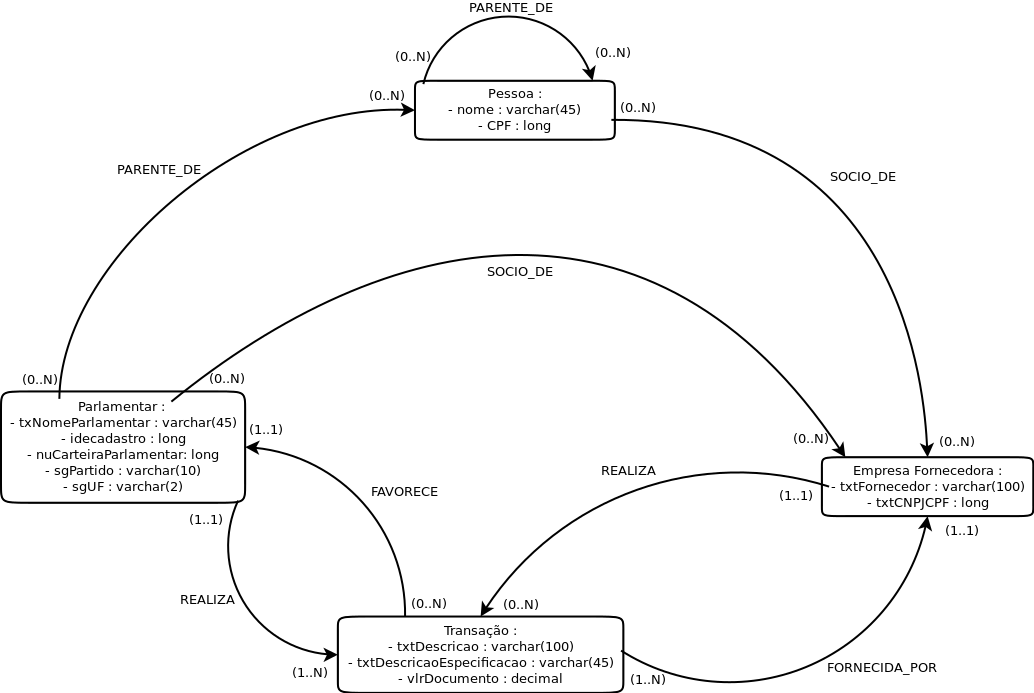
\includegraphics[width=.85\textwidth]{CEAP-v3.png}
\caption{Modelo de dados seguindo o formato GRAPHED}
\label{fig:modeloDeDados}
\end{figure}

Como podemos observar na Figura \ref{fig:modeloDeDados}, existem quatro classes que representam as instâncias dos vértices no banco de dados, que são: Parlamentar, Transação, Empresa fornecedora e Pessoa. As setas que saem de uma classe a outra, representa um relacionamento entre essas classes, que no grafo será representado por uma aresta. Dessa forma, uma instância de um parlamentar, realiza transações, que por sua vez é fornecida por uma empresa fornecedora. Esse caminho descrito, representa as transações da CEAP, fornecida pela Câmara dos Deputados.

De forma análoga, uma empresa fornecedora realiza transações, que por sua vez favorece um certo parlamentar. Esse caminho representa os dados das doações das empresas para os deputados nas eleições de 2014, fornecido pelo TSE. 

Os demais relacionamentos, como "socio-de" e "parente-de" tem por objetivo identificar possíveis fraudes na CEAP, uma vez que um parlamentar não pode utilizar a verba da CEAP com serviços de uma empresa que é sócio. Esses dois caminhos, se apresentaram como o maior desafio para o desenvolvimento do trabalho, uma vez que dados de parentesco dos parlamentares não são dados abertos.

\subsection{ETL} \label{etl-subsection}

	O termo ETL vem do inglês \textit{Extract Transform Load}, e corresponde a \textit{softwares} que tem como função:
\begin{itemize}
		\item Extrair os dados de uma determinada fonte.
		\item Transformar os dados de forma que atendam os requisitos da aplicação.
		\item Carregar os dados no banco de dados.
\end{itemize}
	
	Os dados estão presentes em diferentes formatos: \textit{XML}, \textit{JSON}, \textit{CSV} e \textit{XLSX}. Nesse trabalho foi utilizado o formato \textit{CSV} do ano de 2017. Nesse arquivo \textit{CSV}, os dados estão organizados da seguinte forma:

\begin{table}[H]
\centering
\begin{tabular}{|l|l|l|l|l}
\cline{1-4}
txNomeParlamentar                                 & idecadastro                                       & nuCarteiraParlamentar                             & ... &  \\ \cline{1-4}
ABEL MESQUITA JR.                                 & 178957                                            & 1                                                 & ... &  \\ \cline{1-4}
\begin{tabular}[c]{@{}l@{}}.\\ .\\ .\end{tabular} & \begin{tabular}[c]{@{}l@{}}.\\ .\\ .\end{tabular} & \begin{tabular}[c]{@{}l@{}}.\\ .\\ .\end{tabular} & ... &  \\ \cline{1-4}
ADAIL CARNEIRO                                    & 178864                                            & 92                                                & ... &  \\ \cline{1-4}
\end{tabular}
\caption{Organização dos dados da CEAP}
\label{CEAP-ORG}
\end{table}

	Os dados estão dispostos em linhas e colunas, cada linha representa uma transação diferente para um certo parlamentar. Dentre as colunas disponibilizadas, foram utilizadas as seguintes informações para a fase de extração: TxtDescricao, TxtDescricaoEspecificacao, VlrDocumento, TxNomeParlamentar, IdeCadastro, NumCarteiraParlamentar, SgUF, SgPartido, TxtFornecedor e TxtCNPJCPF. Após o desenvolvimento do modelo de dados, foi desenvolvido um ETL utilizando a linguagem java, para extrair, transformar e carregar os dados para o OrientDB. O OrientDB foi desenvolvido na linguagem java, e executa portanto na JVM. Por esse motivo, o ETL foi feito em java, uma vez que, o OrientDB possui uma boa interface com essa linguagem. O ETL pode ser acessado por meio desse link no github\footnote{https://github.com/gabrielmm1234/CEAP-ETL}.
	
	O fluxo do ETL é exemplificado na Figura \ref{fig:etlfluxo}. Dessa forma o fluxo se organiza em ler linha a linha do csv fornecido pela Câmara dos Deputados, e criar os vértices e arestas com base em certas condições. Por exemplo, não se pode ter mais de um vértice representando um parlamentar, mas no arquivo fornecido existem diversas transações para um mesmo deputado. Ao ler uma nova linha é preciso saber se estamos tratando de um parlamentar já persistido ou de um novo parlamentar antes de criar o vértice que o representa. O mesmo pensamento ocorre no caso de empresas fornecedoras, uma vez que não se pode ter dois vértices representando uma mesma empresa.
	
\begin{figure}[H]
\centering
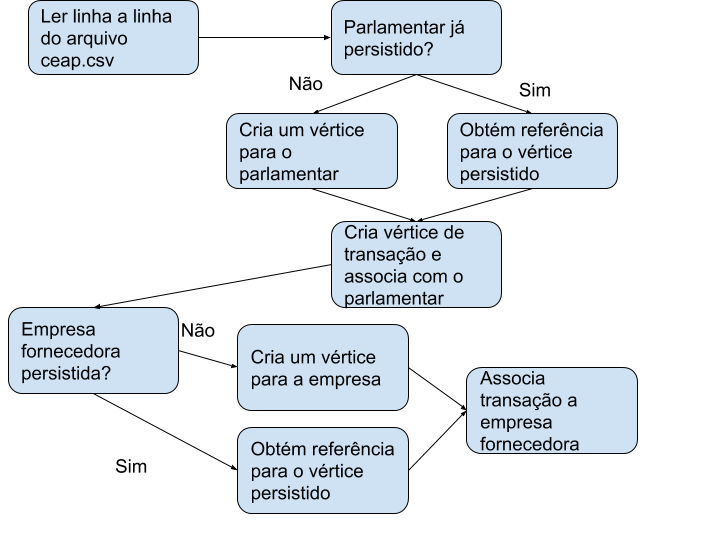
\includegraphics[width=.5\textwidth]{etlfluxo.png}
\caption{Fluxo de extração, transformação e carregamento para o OrientDB}
\label{fig:etlfluxo}
\end{figure}

O ponto chave desse processo são as associações entre os parlamentares com as transações e as empresas que forneceram o serviço. Criando esse vínculo, é possível por meio de consultas de casamento de padrões identificar possíveis fraudes ou padrões de transação e doação envolvendo um mesmo parlamentar e uma mesma empresa. A estrutura de um grafo fornece naturalmente os relacionamentos de forma simples e intuitiva, sendo uma ótima alternativa a estrutura relacional, que é muito comum atualmente. Além disso, a visualização da informação se torna mais clara e objetiva o que é uma ótima característica ao se tratar de transparência em dados governamentais.

O arquivo de dados da CEAP no ano de 2017 possui um total de 209496 transações, o carregamento total dessas transações levou cerca de 16 horas em um notebook com Ubuntu 16-04 LTS, Intel Core i5-5200U CPU 2.20GHz * 4 e 6 Gb de memória RAM. Esse tempo poderia ser otimizado, pois da forma que o ETL foi feito sempre é feito uma busca no banco de dados para saber se um parlamentar ou empresa já estão persistidos. Como o tempo de carga não é um objetivo prioritário no escopo do projeto essa melhora no tempo de carregamento não foi feita.

Já o arquivo das doações passou por um processo de filtragem, para obter somente os dados referentes aos deputados federais dos estados de Minas Gerais e Distrito Federal. Esse filtro para obter deputados federais dos dois estados foi feito para validar mais rapidamente a arquitetura e proposta de solução, no futuro demais estados serão adicionados no banco de dados. O arquivo já filtrado possui um total de 19302 doações de empresas a candidatura de diversos deputados. Claramente, somente alguns desses deputados foram de fato eleitos, e portanto deputados que não se encontravam na base da CEAP foram ignorados. O tempo total de processamento desse arquivo foi de 5 horas, podendo ser melhorado nos mesmos princípios dos dados da CEAP.

\section{Consultas para detecção de fraudes}

Finalizado a obtenção e carregamento dos dados no OrientDB, foram feitas consultas em busca dos relacionamentos entre as empresas doadoras e os deputados de Minas Geras e Distrito Federal que utilizaram a CEAP com essas mesmas empresas. O OrientDB possui uma linguagem de consulta baseada na linguagem SQL, diferentemente de outros SGBD orientado a grafos como o Neo4J, que possui uma linguagem própria conhecida como Cypher.
	
	A consulta feita para obter os resultados esperados, é baseada no conceito de casamento de padrão, muito comum em linguagens funcionais. Dessa forma, para obter um certo padrão dentro do grafo o OrientDB fornece a função MATCH, como mostra a Consulta \ref{lst:label}.

\begin{lstlisting}[label={lst:label}, caption={Consulta de relacionamento de doações entre deputados e empresas},captionpos=b, language=sql]
MATCH 
  {class:Parlamentar, as:p} -RealizaTransacao-> 
  	{class:Transacao, as:t} 
       -FornecidaPor-> {class:EmpresaFornecedora, as:e},
  {as:e} -RealizaTransacao-> {class:Transacao, as:t2} 
  	   -FornecidaPara-> {as:p}
RETURN $elements
\end{lstlisting}

A Consulta \ref{lst:label} busca um certo padrão dentro do banco de dados. Esse padrão é definido por parlamentares chamados de "p", que realizam transações da CEAP "t", fornecidas por uma certa empresa "e". Além disso essa mesma empresa "e", realiza uma transação de doação "t2", que é fornecida para o mesmo parlamentar "p" definido no início da sentença. O resultado dessa consulta nos deputados de Minas Gerais e Distrito federal é apresentado na Figura \ref{fig:ceap_tse_graph}

\begin{figure}[H]
\centering
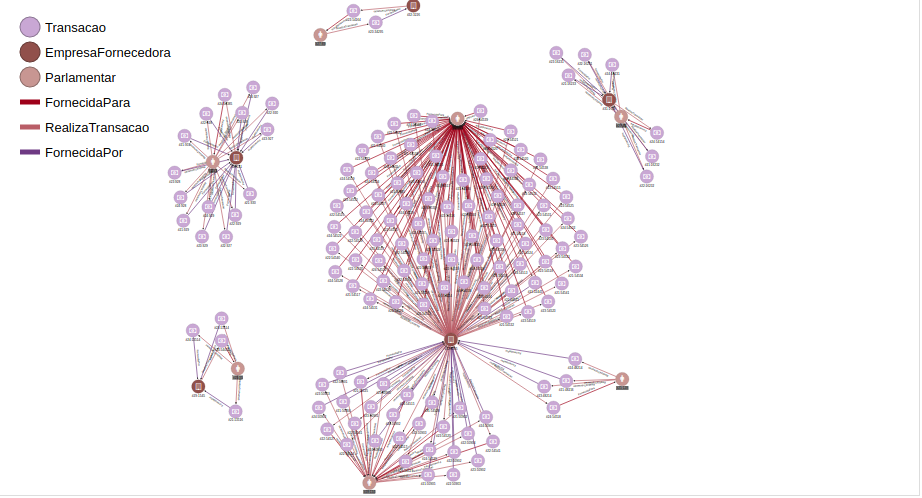
\includegraphics[width=.85\textwidth]{ceap_tse_graph.png}
\caption{Resultado do cruzamento entre dados da CEAP e do TSE.}
\label{fig:ceap_tse_graph}
\end{figure}

\begin{figure}[H]
\centering
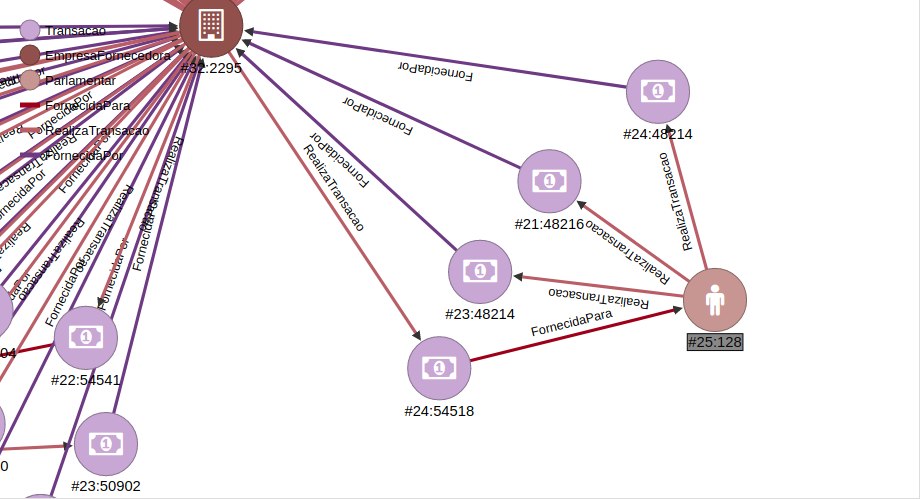
\includegraphics[width=.85\textwidth]{padrao_ceap_tse.png}
\caption{Padrão de relacionamento entre dados da CEAP e do TSE.}
\label{fig:padrao_ceap_tse}
\end{figure}

O padrão definido foi encontrado para um total de sete parlamentares todos em Minas Gerais. A Figura \ref{fig:padrao_ceap_tse} mostra em mais detalhes como o padrão é definido.A partir da orientação das setas, é possível perceber que o parlamentar representado pelo vértice marrom claro e com o ícone de uma pessoa, realizou três transações, representadas pelo vértice roxo claro, com uma certa empresa representada pelo vértice marrom escuro. Sendo que essa empresa fez uma doação para esse parlamentar. No total, foram 44 transações registradas na CEAP, e 96 doações registradas pelo TSE que estão seguindo esse padrão.

Foi feita uma consulta para obter os padrões que podem ser considerados fraudes na CEAP, e testada com dados fictícios. No caso a consulta busca por deputados que usaram a CEAP com empresas das quais são sócios, como apresentada na consulta \ref{lst:label2}.

\begin{lstlisting}[label={lst:label2}, caption={Consulta de relacionamento de uso da CEAP entre deputados e empresas nas quais o deputado é sócio.},captionpos=b, language=sql]
MATCH 
  {class:Parlamentar, as:p} -RealizaTransacao-> 
  	{class:Transacao, as:t} 
    	-FornecidaPor-> {class:EmpresaFornecedora, as:e},
  {as:p} -Socio_De-> {as:e}
RETURN $elements
\end{lstlisting}

\begin{figure}[H]
\centering
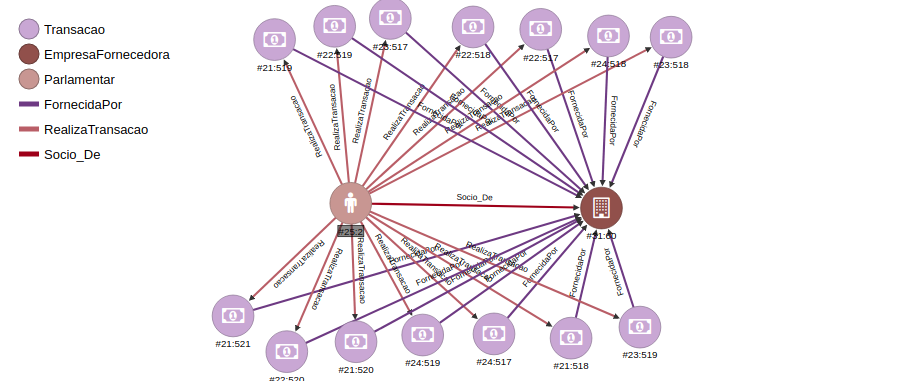
\includegraphics[width=.85\textwidth]{socios.png}
\caption{Padrão de uma transação fraudulenta com dados fictícios.}
\label{fig:socios}
\end{figure}

Como mostra a Figura \ref{fig:socios}, a consulta consegue localizar um padrão de transações efetuadas entre um deputado e uma empresa, na qual o deputado faz parte do quadro de sócios. A forma com que o grafo é apresentado visualmente, pode facilitar bastante o entendimento dos relacionamentos, de forma que fica claro que um deputado, representado pelo círculo com o ícone de uma pessoa, é sócio de uma empresa que prestou serviços com o dinheiro da CEAP. Dessa forma, a visualização gráfica, é uma das vantagens de um SGBD orientado a grafos, pois, a visualização dos vínculos em um grafo é mais simples e intuitiva do que uma estrutura de tabela utilizada nos SGBD relacionais.

\section{Sistema Web}

\section{Conclusão}